\documentclass[20pt]{report}
\usepackage{graphicx}
\usepackage{caption}
\usepackage{relsize}
\usepackage{listings}
\usepackage{textcomp}
\usepackage{hyperref}
\usepackage{wasysym}
\usepackage{verbatim}
\usepackage{color}

\title{How to Write\\
Research Papers in Computer Science}
\author{Bishwajit Saha \\
		Student ID: 1205043\\
		Dept: CSE \\
		Sec: A
		}
\date{\today}


\begin{document}
  \maketitle
  \begin{abstract}
  This report tells all the process for writing a nice and worthy thesis paper,research paper or report.For publishing research papers in a well-known scientific magazines,that research papers must be well written.And this report says exactly that by using latex environment.One must follow the rules that have discussed here for writing a good research paper.
  \end{abstract}
  \tableofcontents
  
  
  \chapter{Research in Computer Science and Engineering}
  \paragraph{In Computer Science and Engineering research is the starting step of inventing new revolution.No big job comes without research.But at the time of research one should follow some rules.Otherwise research may be lengthy or may not bring any good result. \\Steps to follow:}
  \begin{itemize}
  \item Study and explore your area of interest.
computer science and engineering;
  \item Choose a research problem.
  \item Find one or two co-researchers and form a research group.
 \item Read related research papers published in good journals
and conferences and present those papers in the group, by
rotation.
 \item Sit frequently for brainstorming on the problem and try to
find non-trivial results.
\item Find good results around the problem and write papers.
  \end{itemize} 
 
\begin{figure}[!htbp]
\begin{center}
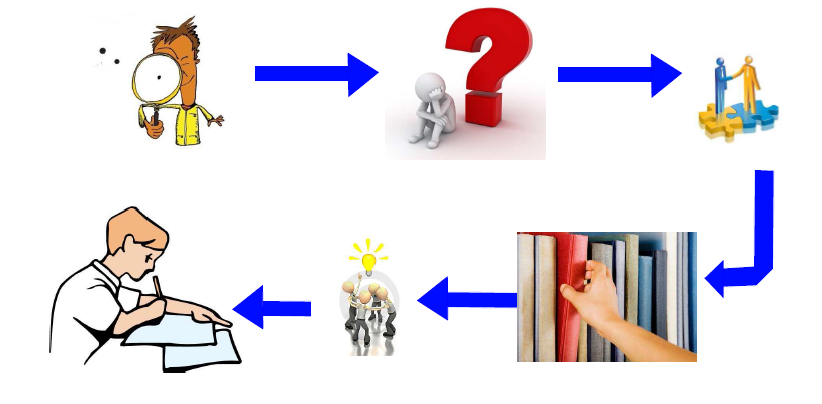
\includegraphics[scale=0.8,natwidth=197,natheight=248]{image.png}%if you compile using latex you will have to provide natwidth and natheight, however, still the produced dvi won't have the image in it, :-( you will have to then convert dvi to pdf using dvipdfm, in the pdf, png/jpg image will be shown, good thing is that pdflatex will work even without natwidth, natheight, :-) 
\caption{Steps to follow}
\label{fig:image}
\end{center}
\end{figure}

  \chapter{Writing a Paper}
 \paragraph{After research it is very important to write a good research paper.Howover writing a good research paper is not so easy.One should follow some important terms when writing a research paper.It includes various terms.These are illustrated below.} 
  \section{Organization of a Research Paper}
  \paragraph{It is the whole image of a good research paper.It includes all the terms that are strongly needed to write a good research paper.\\Here are the terms: }
  \begin{enumerate}
  \item Title
  \item Author/Authors Name and Affiliation
\item Abstract and Key words
\item Introduction
\item Preliminaries / Background / Related Works
\item Main Results (may be several sections)
\item Conclusions
\item Acknowledgement
\item References
\item Appendix
  \end{enumerate}
  
 \section{Title of a Paper} 
 \paragraph{It must contain the following terms: }
 \begin{enumerate}
  \item The title should convey some information to the reader.
  \item The title should tell the reader exactly what the paper is
about and, further, what points it makes.
  \end{enumerate} 
  
  \section{Authors Name}
   \textbf {Name}: At the beginning of your career, pick a name for yourself
and stick to it.\\
Md. Saidur Rahman\\
M. S. Rahman\\
Md. S. Rahman
  \begin{center}
\begin{tabular}[t]{|p{0.5\textwidth}|p{0.4\textwidth}|}
\hline
\begin{center}
\textcolor{red}{Wrong}
\end{center}  & \begin{center}
\textcolor{green}{Correct}
\end{center} \\
\hline
\textcolor{red}{Dr.} Md. Saidur Rahman & Md. Saidur Rahman\\
\hline
\textcolor{red}{Prof.} Md. Saidur Rahman & Md. Saidur Rahman\\
\hline
\end{tabular}
\end{center}

 \section{Affiliation}
   \textbf {Affiliation:} \\
   Organization, Postal Address and Email Address
  \begin{center}
\begin{tabular}[t]{|p{0.3\textwidth}|p{0.5\textwidth}|}
\hline
Bad & Good \\
\hline
\textcolor{red}{Professor} & Dept. of Computer Science and Engineering\\
\hline
Dept. of CSE & BUET, Dhaka 1000\\
\hline
\hline
BUET, Dhaka 1000 & Bangladesh\\
\hline
\end{tabular}
\end{center}

\section{Abstract}
\paragraph{ Write the full paper in a concise form (at most ten lines.)
It should contain}
\begin{itemize}
\item \textbf {Motivation}: Why do we care about the problem and the
results?
\item \textbf {Problem statement}: What problem is the paper trying to
solve and what is the scope of the work?
\item \textbf {Approach}: What was done to solve the problem?
\item \textbf {Results}: What is the answer to the problem?
\item \textbf {Conclusions}: What implications does the answer imply?
\end{itemize}
\textbf{General features of an abstract:}
\begin{itemize}
\item self contained.
\item should not make any bibliographic reference.
\item should contain a minimum number of notations.
\end{itemize}

\section{Key Words}
\paragraph{The key words are provided so that}
\begin{itemize}
\item editor can choose appropriate reviewer.
\item archiving services can place your paper correctly into a
database.
\end{itemize}
  \begin{center}
\begin{tabular}[t]{|p{0.2\textwidth}|p{0.3\textwidth}|}
\hline
\textcolor {red} {Bad Choice} & \textcolor {blue} {Good Choice} \\
\hline
New & Algorithm\\
\hline
Intersting & Sperating Triangle\\
\hline
\hline
Optimal & Matching\\
\hline
\end{tabular}
\end{center}

\section{Introduction}
\paragraph{ Write the full paper in 2-3 pages. Most difficult part of a paper.
This is the first section of a paper but the last section to
complete.}
\begin{description}
  \item[**   ] make general statements about the problem related
subject and define the problem.
\item[**   ] bring out the importance of the problem from theoretical
and application point of view.
\item[**  ] present an overview on the history and current research on
the problem. Justify a research gap for your study.
\item[**  ] continue a tradition, or propose a completely new
approach.
\item[**  ] sketch the intent of your own work and outline important
characteristics and results of your own work.
\item[**  ] give an outline of the organization of the paper.
\end{description}

\section{Organization of your paper}
\paragraph{It is provided so that}
\begin{itemize}
\item Plan your sections and subsections. Use a top-down
writing method. Use a sentence to represent the points
(paragraphs) in each subsections.
\item Writing details: expand a sentence in the sketch into a
paragraph.
\item Keep a logical flow from section to section, paragraph to
paragraph, and sentence to sentence.
\end{itemize}

\section{Preliminaries}
\paragraph{To make the paper self-contained}
\begin{itemize}
\item Define the notations and definitions that will be used
throughout the paper.
\item Describe briefly the known methods that you will use in
your method.
\item State the known results as Lemmas that you will use for
proving your result.
\item Describe your preliminary results.
\end{itemize}

\section{Main Results}
\paragraph{It is very important to organize a good research paper.The research paper should be written in a way so that one can easily understand when writing it and doesn't get bored.\\To make a paper good looking and attracting :}
\begin{itemize}
\item Plan your sections and subsections to present your main
results.
\item Give short and informative section names.
\item Give a brief outline at the beginning of each section.
\item Give intuitive idea and outline of every proof and method,
and then give the details.
\item Keep a logical flow from section to section, paragraph to
paragraph, and sentence to sentence.
\end{itemize}

\section{Conclusions}
\paragraph{It is an important part of writing a good research paper.In this section one should not elaborate his/her whole research paper rather should give a brief description about his/her research.\\To make it standard follow :}
\begin{itemize}
\item Restate your contribution.
\item Mention any useful implication of your results that have not
mentioned earlier.
\item Mention future direction of research and interesting open
problems that you have found in doing this research work.
\end{itemize}

\section{Acknowledgement}
\paragraph{It is also a very important part.When you start to write a paper you may need information from other sources.\\So,}
\begin{itemize}
\item Give thanks to anonymous reviewers and to persons who
helped you in doing this work.
\item Acknowledge grants or support that you have received for
doing this work.
\end{itemize}

\section{Bibliographic References}
\paragraph{At the time of writing a paragraph you should mention the references or bibliographies from those you have taken help.\\For these the following rules should be followed.}
\begin{itemize}
\item Reference or Bibliography?\\
%\begin{verse}
 \textcolor {blue} {References:}List of sources that you actually cite in your
paper.\\
\textcolor {blue} {Bibliography}: List of all related publications.
 %\end{verse}
\item Follow same style for all references.
\item Each item in the list must have at least the following fields:
Author(s), Title, Journal or Proceedings, Publisher, Page
Numbers, Year.
\item URLs do not have a publication date, hence say when
accessed it last.
\item Follow the style specified by the publisher.
\end{itemize}

\section{Appendix}
\paragraph{It is a part which may bring whole of your paper within a glance.}
\begin{itemize}
\item Bring the materials from main chapters to Appendix which
obstruct the flow and smoothness of the paper.
\end{itemize}

\section{What To Do Once The Paper Is Written?}
\paragraph{After writing a research paper you should revise this many times.Then you can submit it in a good journal or conference.But You must follow the rules of those journals/conferences at where you submit it.This process may be sometimes lengthy.You should follow the following rules until your research paper is not accepted by a good jounal.}
\begin{itemize}
\item Revise the paper several times. How many times?
\item Submit the paper to a conference/journal.
\item Receive review report.
\item Revise the paper according to reviewers comments and
improve your results.
\item Resubmit the revised version.
\item Repeat the process until the paper is accepted.
\item Send your source files to publishing house together with
copyright transfer.
\item Check the galley proof of the paper carefully when you
receive it.
\end{itemize}


  \chapter{Writing a Thesis}
  \paragraph{Writing a thesis paper is almost the same process of writing a rsearch paper.It includes Title page,table of contents,abstract list of figures etc.abstract should be one page. }
  \section{Thesis Organization}
  \paragraph{This contains the terms of writing a thesis paper.\\They are :}
  \begin{enumerate}
  \item \textcolor {blue} {Title Page}
  \item \textcolor {blue} {Table of Contents}
  \item \textcolor {blue} {Abstract} (One page)
  \item \textcolor {blue} {List of Figures, List of Tables}
  \item \textcolor {blue} {Chapter 1:}\begin{verse}
  Introduction (5-10 pages).
  \end{verse}
   \item \textcolor {blue} {Chapter 2:}\begin{verse}
  Preliminaries / Background / Related Works (8-20
pages).
  \end{verse}
  \item \textcolor {blue} {Chapter 3-5:}\begin{verse}
  Main Contents. Each chapter contains a result in
theoretical thesis. For applied/experimental area
these chapters are on Modeling, Methodologies,
Experimentation, Results and Discussions.
  \end{verse}
  \item \textcolor {blue} {Chapter 6:}\begin{verse}
  Conclusions and Future Work ( 3-6 pages).
  \end{verse}
  \item \textcolor {blue} {Appendix}
  \item \textcolor {blue} {Bibliography}
  \item \textcolor {blue} {Index}
  \end{enumerate}
  

\chapter{Writing Tools}
\paragraph{There are several writing tools for writing your research paper.You may use these tools when you write the research paper.It will make easy for you to write these and will give a good shape of your research paper.}
\begin{enumerate}
\item \textcolor {blue} {LaTex: }For typesetting of text.
\item \textcolor {blue} {LatexDraw: }For drawing figures.
\item \textcolor {blue} {Xfig: }For drawing figures.
\end{enumerate}
\paragraph{ LaTex templates for submission to journals are available in
journal web pages.\\
You can also find LaTex thesis templates in Internet.}

\chapter{Plagiarism}
\paragraph{When writing a research paper it is a great shy stealing ideas from others or copying other sources.It will make your research paper the worst one.You may loose honourity.This is strongly prohibited when writing a research paper.}
\section{What is Plagiarism}
\paragraph{Here are the things :}
\begin{enumerate}
\item Copying from other source.
\item Stealing other’s idea.
\item Never do it. It can spoil your career.
\end{enumerate}
\begin{center}
\emph{{\Large You may need to mention works of others, use method of
others.\\What will you do?}}

\end{center}
\begin{verse}
1. Read and understand the work.
\end{verse}
\begin{verse}
2. Write in your own word (do not use verbatim copy)
\end{verse}
\begin{verse}
3. Explain with your own illustrative figures
\end{verse}
\begin{verse}
4. Give proper citation
\end{verse}
Your own work/results should be significantly different from the
cited work. You cannot use other’s works as the major content
of your paper.

\chapter{Review Report and Revision Report}
\section{Review Report}
\paragraph{ Writing a review report is a professional duty. Usually it a
voluntary work.
A review report should contain}
\begin{itemize}
\item Problem statement
\item Contribution of the paper
\item Strength and weakness of the paper
\item Your recommendation
\item Comments to author for improvement of the paper
\end{itemize}
\section{Revision Report}
\paragraph{ A revision report should contain}
\begin{itemize}
\item Thanks to the anonymous referees
\item Your comments and action addressing each point raised by
the reviewers.
\end{itemize}

\chapter{Concluding Remarks}
\paragraph{You should always remember that publishing a good research paper is far better than publishing hundreds of poor papers.You should write quality research paper.\\You should follow: }
\begin{enumerate}
\item Always try to do quality research.
\item One good publication is better than dozens of poor
publications.
\item You cannot regain your reputation by publishing 20 good
publications if you damage your image by publishing only
one bad paper.
\item Do not publish review/survey paper unless you are an
expert of the field.
\end{enumerate}
\begin{center}
\emph {\textbf {Publish your research results in good journals.\\}}
\emph{\textbf{But do not publish a journal !!!!}}
\end{center}

\chapter{Acknowledgement}
\paragraph{At last you should mention the sources you have used to fulfill your research paper.It is a very important part of research paper.You should follow like below :}
\begin{itemize}
\item Sources:
\begin{itemize}
\item D. E. Knuth, T. Larrabee and P. M. Robers, Mathematical
Writing, MAA Notes, 14, The Mathematical Association of
America, 1989.
\item S. G. Krantz, A primer of Mathematical Writing, American
Mathematical Society, 1997.
\item R. Andonie and I. Dzitac, How to write a good paper in
computer science and how will it be measured by ISI web of
knowledge, Int. J. of Computers, Communications and
Control, 4, pp. 432-446, 2010.
\item U. Khedker, How to Write a Good Paper? Indian Institute of
Technology, Bombay (slides).
\item https://cs.uwaterloo.ca/ brecht/thesis-hints.html, accessed
on August 29, 2013.
\end{itemize}
\end{itemize}
\end{document}
